%%
%%

\chapter{Qu'est-ce que Bacula ?}
\label{_ChapterStart41}
\index[general]{Qu'est-ce que Bacula ? }
\index[general]{Bacula!Qu'est-ce que }
\addcontentsline{toc}{section}{Qu'est-ce que Bacula ?}

{\bf Bacula} est un jeu de programmes qui vous permet (ou \`a l'administrateur
syst\`eme) de faire des sauvegardes, restaurations, et v\'erifications des
donn\'ees d'un ordinateur sur un r\'eseau h\'et\'erog\`ene. Bacula peut  
fonctionner compl\`etement sur un seul ordinateur. Il est capable de 
sauvegarder sur des supports vari\'es, y compris disques et cartouches.

En termes
techniques, il s'agit d'un programme de sauvegarde Client/Serveur. Bacula est
relativement facile d'utilisation et efficace, tout en offant de nombreuses
fonctions avanc\'ees de gestion de stockage qui facilitent la recherche et la
restauration de fichiers perdus ou endommag\'es. Gr\^ace \`a sa conception
modulaire, Bacula est \'echelonnable depuis le simple syst\`eme constitu\'e
d'un ordinateur, jusqu'au syst\`eme de plusieurs centaines d'ordinateurs
diss\'emin\'es sur un vaste r\'eseau. 

\section{Qui a besoin de Bacula ?}
\index[general]{Qui a besoin de Bacula ? }
\index[general]{Bacula!Qui a besoin de }
\addcontentsline{toc}{section}{Qui a besoin de Bacula ?}

Si vous utilisez actuellement un programme tel que {\bf tar}, {\bf dump}, ou
{\bf bru} pour sauvegarder vos donn\'ees, et aimeriez une solution r\'eseau,
plus de flexibilit\'e, ou les commodit\'es d'un catalogue, Bacula vous
procurera certainement les fonctions suppl\'ementaires que vous recherchez.
Cependant, si vous avez peu d'exp\'erience des syst\`emes Unix ou si vous
n'avez pas l'exp\'erience d'un syst\`eme de sauvegarde sophistiqu\'e, nous ne
vous recommandons pas l'utilisation de Bacula, car il est beaucoup plus
difficile \`a installer et utiliser que {\bf tar} ou {\bf dump}. 

Si vous attendez de Bacula qu'il se comporte comme les programmes simples 
mentionn\'es ci-dessus et qu'il \'ecrive sur toute cartouche ins\'er\'ee dans le 
lecteur, vous \'eprouverez des difficult\'es \`a travailler avec Bacula. Bacula 
est con\c {c}u pour prot\'eger vos donn\'ees en suivant les r\`egles que vous sp\'ecifiez, 
ce qui signifie que la r\'eutilisation d'une cartouche ne se fera qu'en dernier 
ressort. Il est possible de "contraindre" Bacula \`a \'ecraser toute cartouche dans 
le lecteur, mais il est plus facile et plus efficace d'utiliser un outil 
plus basique pour ce genre d'op\'erations.

Si vous utilisez {\bf Amanda} et aimeriez un programme de sauvegarde qui peut
\'ecrire sur plusieurs volumes (qui ne soit pas limit\'e par la capacit\'e de vos
cartouches), Bacula peut certainement satisfaire vos besoins, d'autant que
plusieurs de nos utilisateurs estiment que Bacula est plus simple \`a
installer et utiliser que d'autres programmes \'equivalents. 

Si vous utilisez actuellement un logiciel commercial sophistiqu\'e tel que
{\bf Legato Networker}, {\bf ARCserveIT}, {\bf Arkeia}, ou {\bf
PerfectBackup+}, vous pourriez \^etre interess\'e par Bacula qui fournit la
plupart de leurs fonctions et qui est un logiciel libre sous licence GNU
version 2. 

\section{Composants ou Services de Bacula}
\index[general]{Bacula!Composants ou Services de }
\index[general]{Composants ou Services de Bacula }
\addcontentsline{toc}{section}{Composants ou Services de Bacula}

Bacula est constitu\'e des cinq composants ou services majeurs suivants : 

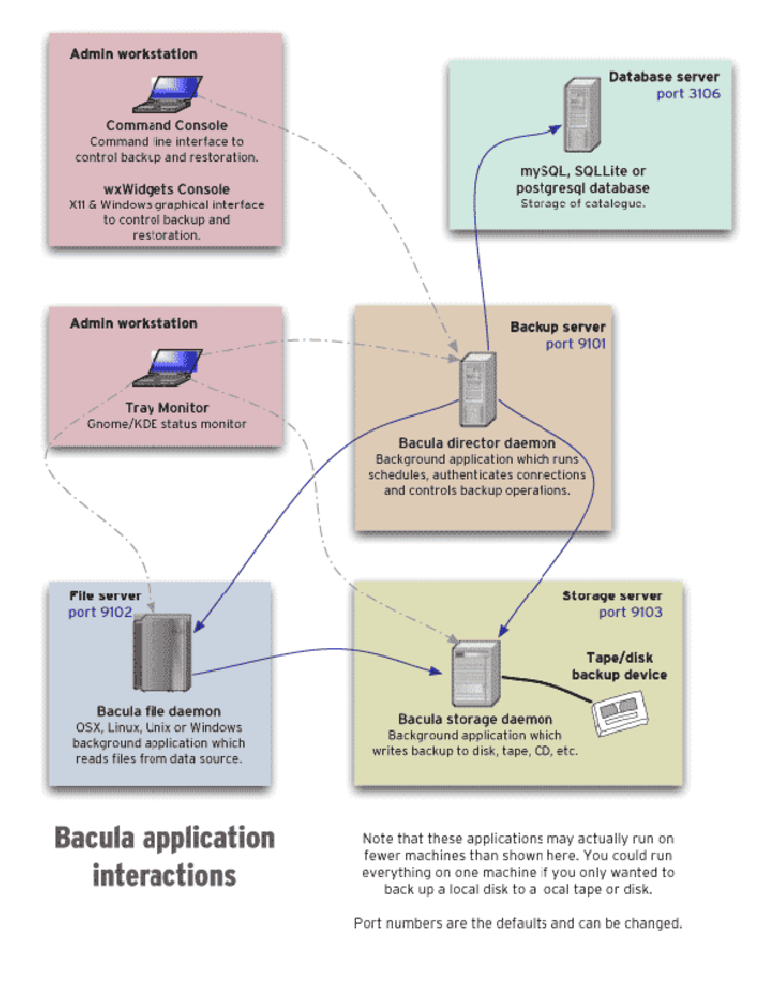
\includegraphics{./bacula-applications.eps} 
(remerciements \`a Aristedes Maniatis pour ce sch\'ema et le suivant) 

\begin{itemize}
\item 
   \label{DirDef}
   Le service {\bf Bacula Director
\label{a1}
} est le programme qui supervise toutes  les op\'erations de sauvegarde,
restauration, v\'erification et archivage.  L'administrateur syst\`eme utilise
le Bacula Director pour planifier les  sauvegardes et restaurer les fichiers.
Pour plus de d\'etails, consultez la section concernant la conception du Daemon Director 
dans la documentation pour d\'eveloppeurs. Le Director est ex\'ecut\'e en tant que {\it daemon} 
ou service (c'est \`a dire en t�che de fond).
\item 
   \label{UADef}
   Le service {\bf Bacula Console} est le programme qui permet \`a 
l'administrateur ou \`a l'utilisateur de communiquer avec le {\bf Bacula 
Director} (voir ci-dessus). Actuellement, le service Bacula Console  est
disponible en trois versions. La premi\`ere et la plus simple est 
d'ex\'ecuter le programme Console dans une fen\^etre shell (i.e. interface
TTY).  La plupart des administrateurs syst\`eme trouveront cette m\'ethode
parfaitement  ad\'equate. La seconde version est une interface graphique GNOME
qui est loin d'\^etre compl\`ete, mais est
tout \`a fait  fonctionnelle puisqu'elle poss\`ede la plupart des
possibilit\'es de la Console  shell. La troisi\`eme version est une interface
graphique wxWidgets qui permet de s\'electionner  interactivement les fichiers
\`a restaurer. Elle int\`egre la plupart des fonctionnalit\'es  de la console
shell, permet la compl\'etion automatique avec la touche tabulation, et 
fournit une aide instantan\'ee relative \`a la commande que vous \^etes en
train de taper.  Pour plus de d\'etails, consultez la section 
\ilink{Conception de la Console Bacula}{_ConsoleChapter} dans la documentation 
pour d\'eveloppeurs. 
\item 
   \label{FDDef}
   Le service {\bf Bacula File} (ou programme client) est le programme install\'e
sur la machine \`a sauvegarder. Il est sp\'ecifique au syst\`eme sur lequel
il est  ex\'ecut\'e et a la charge de fournir les attributs des fichiers et
les donn\'ees  requis par le Director. Les Services File sont aussi charg\'es
de la partie  d\'ependant du syst\`eme de fichiers lors de la restauration des
attributs de  fichiers et des donn\'ees. Pour plus de d\'etails, consultez le
document  sur la conception du File Daemon dans le Guide pour Developpeurs. Ce
programme est ex\'ecut\'e en  tant que service sur la machine \`a sauvegarder,
et la documentation s'y r\'ef\`ere  parfois en tant que Client (par exemple
dans les fichiers de configuration de  Bacula). En plus du File Daemon pour
Unix/Linux, il existe un File Daemon pour  Windows (usuellement distribu\'e au
format binaire). Le File Daemon Windows  fonctionne sur toutes les versions
actuelles de Windows (NT,  2000, XP, 2003 et peut-\^etre aussi 98 et Me). 
\item 
   \label{SDDef}
   Le service {\bf Bacula Storage} est le programme qui transf\`ere les donn\'ees
et  les attributs de fichiers aux m\'edia physiques ou aux volumes et les
restitue  lors de restaurations. En d'autres termes, Le storage Daemon est
responsable  des op\'erations de lecture et d'\'ecriture sur vos cartouches (ou
autres m\'edia  de stockage, comme par exemple des fichiers). Pour plus de 
d\'etails consultez la  Documentation Pour D\'eveloppeurs sur la conception du 
Storage Daemon. 
\item 
   \label{DBDefinition}
   Les services {\bf Catalogue} ont pour t\^ache de maintenir \`a jour la base de
donn\'ees des index de fichiers et volumes pour tous les fichiers
sauvegard\'es.  Les services {\bf Catalogue} permettent \`a l'administrateur
syst\`eme ou \`a  l'utilisateur de localiser rapidement et restaurer n'importe
quel fichier.  Les services Catalogue de Bacula le placent dans une
cat\'egorie diff\'erente  de programmes tels que tar et bru, puisque le
catalogue Bacula maintient  un enregistrement de chaque  volume utilis\'e,
chaque job ex\'ecut\'e et chaque fichier sauvegard\'e  ce qui permet des
restaurations et une gestion de volumes efficaces. Bacula  supporte
actuellement trois bases de donn\'ees diff\'erentes, MySQL, PostgreSQL,  et
SQLite. L'une des trois doit \^etre choisie \`a la compilation de {\bf
Bacula}.  

Les trois bases de donn\'ees actuellement support\'ees (MySQL, PostgreSQL, ou
SQLite)  fournissent de nombreuses fonctions telles l'indexation rapide,
requ\^etes  arbitraires, et s\'ecurit\'e. Bien que nous pr\'evoyions de
supporter d'autres  bases de donn\'ees SQL majeures, l'impl\'ementation
actuelle s'interface seulement  avec MySQL, PostgreSQL, et SQLite. Pour plus
de d\'etails consultez le  
\ilink{document sur la conception des Services Catalogue
}{_ChapterStart30}.  

Les RPMs pour MySQL et PostgreSQL font partie de la distribution Red Hat. 
Sinon, il est tout \`a fait ais\'e de les construire \`a partir des sources. 
Consultez le chapitre 
\ilink{ Installer et configurer MySQL}{_ChapterStart}  ou 
\ilink{ Installer et configurer PostgreSQL}{_ChapterStart10} de
ce  document pour plus de d\'etails. Pour plus d'informations sur MySQL et
PostgreSQL,  consultez 
\elink{www.mysql.com}{http://www.mysql.com} ou 
\elink{www.postgresql.org}{http://www.postgresql.org}.  

Configurer et construire SQLite est encore plus facile. Pour les d\'etails  de
configuration de SQLite, consultez le chapitre 
\ilink{Installer et Configurer SQLite}{_ChapterStart33} de ce
document. 
\item 
   \label{MonDef}
   Le service {\bf Bacula Monitor} est le programme qui permet \`a
l'administrateur  ou \`a l'utilisateur de contr\^oler le statut des {\it
daemons} Bacula ({\bf Bacula Directors},  {\bf Bacula File Daemons} et {\bf
Bacula Storage Daemons}) (voir ci-dessus). Actuellement,  la seule version
disponible est une version GTK+, qui fonctionne avec Gnome et KDE (ainsi  que
tout gestionnaire de fen\^etre qui respecte le standard system tray
FreeDesktop.org). 
\end{itemize}

Pour r\'ealiser avec succ\`es les op\'erations de sauvegarde et restauration,
les quatre services suivants doivent \^etre configur\'es et lanc\'es : le
Director Daemon, le File Daemon, le Storage Daemon et MySQL, PostgreSQL ou
SQLite. 

\section{Configuration de Bacula}
\index[general]{Configuration de Bacula }
\index[general]{Bacula!Configuration de }
\addcontentsline{toc}{section}{Configuration de Bacula}

Pour que Bacula comprenne votre syst\`eme, quels clients vous voulez
sauvegarder et comment, vous devez cr\'eer un certain nombre de fichiers de
configuration. La suite brosse un tableau de ces op\'erations. 

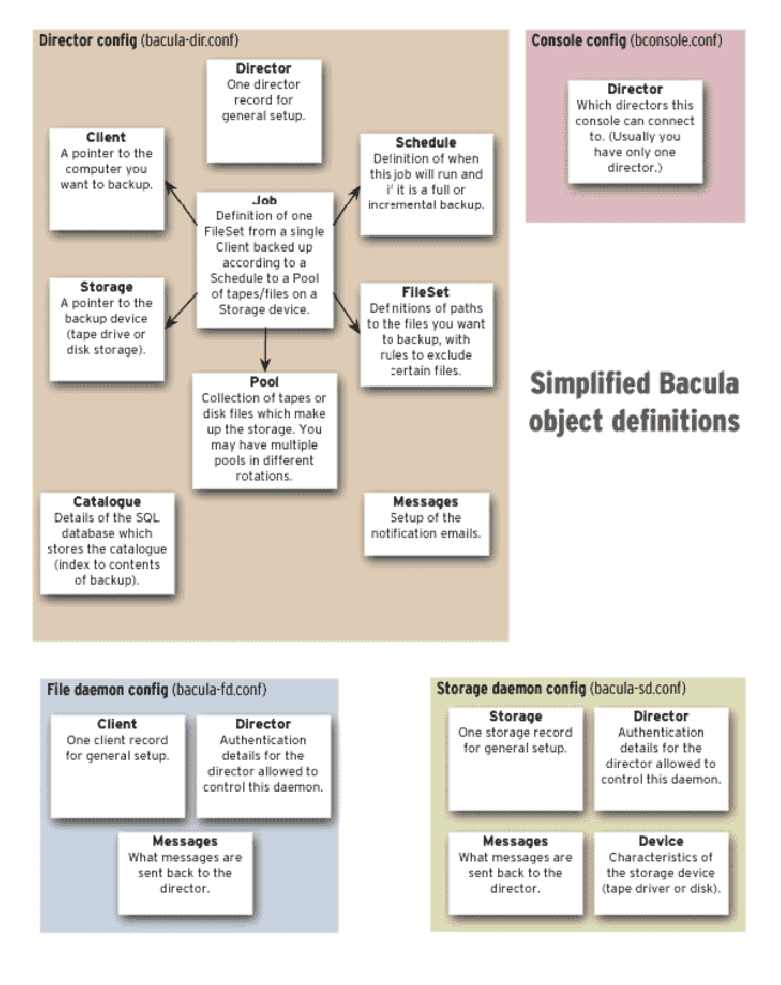
\includegraphics{./bacula-objects.eps} 

\section{Conventions utilis\'ees dans ce document}
\index[general]{Conventions utilis\'ees dans ce document }
\index[general]{Document!Conventions utilis\'ees dans ce }
\addcontentsline{toc}{section}{Conventions utilis\'ees dans ce document}

{\bf Bacula} est en constante \'evolution, par cons\'equent, ce manuel ne sera
pas toujours en accord avec le code. Si un objet de ce manuel est
pr\'ec\'ed\'e d'un ast\'erisque (*), cela signifie que cette fonctionnalit\'e
particuli\`ere n'est pas impl\'ement\'ee. S'il est pr\'ec\'ed\'e d'un signe
plus (+), cela indique que la fonction est peut-\^etre partiellement
impl\'ement\'ee. 

Si vous lisez la version de ce manuel fournie avec les sources de Bacula, le
paragraphe ci-dessus reste vrai. En revanche, si vous lisez la version en
ligne : 
\elink{www.bacula.org/manual}{http://www.bacula.org/manual}, veuillez garder
\`a l'esprit que cette version d\'ecrit la version courante de d\'eveloppement
de Bacula (celle du CVS) qui peut contenir des fonctionnalit\'es qui
n'existent pas dans la version "officielle". De m\^eme, il est
g\'en\'eralement un peu \`a la tra{\^\i}ne derri\`ere le code. 

\section{D\'emarrage rapide}
\index[general]{D\'emarrage rapide }
\index[general]{Rapide!D\'emarrage }
\addcontentsline{toc}{section}{D\'emarrage rapide}

Pour faire fonctionner Bacula rapidement, nous vous recommandons de commencer
par parcourir la section Terminologie ci-dessous, de passer rapidement en
revue le chapitre suivant intitul\'e 
\ilink{L'\'etat actuel de Bacula}{_ChapterStart2}, puis le 
\ilink{Guide de d\'emarrage rapide de Bacula}{_ChapterStart37},
qui vous donnera une vue d'ensemble de la mise en oeuvre de Bacula . Apr\`es
quoi vous devriez poursuivre avec le chapitre sur 
\ilink{ L'installation de Bacula}{_ChapterStart17}, puis le chapitre
\ilink{Comment configurer Bacula}{_ChapterStart16}, et finalement,
le chapitre  \ilink{Ex\'ecuter Bacula}{_ChapterStart1}. 

\section{Terminologie}
\index[general]{Terminologie }
\addcontentsline{toc}{section}{Terminologie}

Pour faciliter la communication autour de ce projet, nous fournissons ici les
d\'efinitions de la terminologie que nous utilisons. 

\begin{description}

\item [Administrateur]
   \index[sd]{Administrateur }
   La ou les personne(s) responsable(s) de l'administration  du syst\`eme Bacula.


\item [Sauvegarde]
   \index[sd]{Sauvegarde }
   Nous utilisons ce terme pour un job Bacula qui sauvegarde des  fichiers. 

\item [Fichier Bootstrap (Bootstrap File)]
   \index[sd]{Fichier Bootstrap (Bootstrap File) }
   Le bootstrap est un fichier ASCII qui  contient, sous une forme compacte, les
commandes qui permettent \`a Bacula ou \`a  l'utilitaire autonome {\bf
bextract} de restaurer les contenus d'un ou plusieurs  volumes, par exemple,
l'\'etat courant d'un syst\`eme qui vient d'\^etre sauvegard\'e.  Avec un
fichier bootstrap, Bacula peut restaurer votre syst\`eme sans catalogue.  Vous
pouvez cr\'eer un fichier bootstrap depuis un catalogue pour extraire le
fichier  que vous voulez. 

\item [Catalogue]
   \index[sd]{Catalogue }
   Le catalogue est utilis\'e pour stocker des informations sommaires  concernant
les Jobs et Clients, les fichiers qui ont \'et\'e sauvegard\'es ainsi que le 
ou les volume(s) o\`u ils ont \'et\'e sauvegard\'es. L'information stock\'ee
dans le  catalogue permet \`a l'administrateur ou aux utilisateurs de
d\'eterminer quels jobs  ont \'et\'e ex\'ecut\'es, leur statut, ainsi que
d'importantes caract\'eristiques de chaque  fichier sauvegard\'e. Le catalogue
est une ressource en ligne, mais ne contient pas  les donn\'ees pour les
fichiers sauvegard\'es. La plupart des informations stock\'ees  dans le
catalogue le sont aussi sur les volumes de sauvegarde (i.e. cartouches).  Bien
sur, les cartouches auront aussi une copie du fichier en plus de ses attributs
 (voir ci-dessus).  

La fonction Catalogue est de celles qui distinguent Bacula de simples
programmes  de sauvegarde et archivage tels que {\bf dump} et {\bf tar}. 

\item [Client]
   \index[sd]{Client }
   Dans la terminologie de Bacula, le mot Client d\'esigne une machine 
sauvegard\'ee, et est synonyme de File service ou File Daemon. Nous nous y
r\'ef\'erons  assez souvent par "le FD". Un client est d\'efini dans une
ressource de fichier de  configuration. 

\item [Console]
   \index[sd]{Console }
   Le programme qui interface le Director, permettant \`a  l'administrateur de
contr\^oler Bacula. 

\item [Daemon]
   \index[sd]{Daemon }
   Terminologie Unix pour un programme toujours pr\'esent en arri\`ere plan  pour
prendre en charge une t\^ache donn\'ee. Sur les syst\`emes Windows, ainsi que
certains  Linux, les {\it daemons} sont appel\'es {\bf Services}. 

\item [Directive]
   \index[sd]{Directive }
   Le terme directive est utilis\'e pour d\'esigner une entr\'ee ou
enregistrement \`a l'int\'erieur d'une ressource dans un fichier de 
configuration qui d\'efinit un \'el\'ement sp\'ecifique. Par exemple, la
directive  {\bf Name} d\'efinit le nom de la ressource. 

\item [Director]
   \index[sd]{Director }
   Le principal {\it daemon} serveur de Bacula qui planifie et dirige  toutes
les op\'erations de Bacula. Occasionnellement, nous le d\'esignons par "le
DIR". 

\item [Differentielle (Differential)]
   \index[sd]{Differentielle (Differential) }
   Une sauvegarde qui inclut tous les fichiers  modifi\'es depuis le lancement de
la derni\`ere sauvegarde compl\`ete (Full).  Notez que d'autres logiciels de
sauvegarde peuvent d\'efinir ceci diff\'eremment.  

\item [Attributs de fichiers]
   \index[sd]{Attributs de fichiers }
   Les Attributs de fichiers sont toutes les  informations n\'ecessaires au sujet
d'un fichier pour l'identifier, et toutes ses  propri\'et\'es telles taille,
date de cr\'eation, date de modification, permission, etc.  En principe, les
attributs sont int\'egralement manipul\'es par Bacula de sorte que 
l'utilisateur n'a jamais \`a s'en pr\'eoccuper. Les attributs n'incluent pas
les donn\'ees  du fichier. 

\item [File Daemon]
   \index[sd]{File Daemon }
   Le {\it daemon} ex\'ecut\'e sur l'ordinateur client \`a sauvegarder. Il est 
aussi d\'esign\'e par Service Fichier (File Service) et parfois Service Client
ou FD. 

\item [
   \label{FileSetDef}
   FileSet]
\index[sd]{a name }
Un FileSet est une ressource d'un fichier de configuration qui  d\'efinit les
fichiers \`a sauvegarder. Il consiste en une liste de fichiers ou 
r\'epertoires inclus, une liste de fichiers ou r\'epertoires exclus et la
fa\c{c}on dont les  fichiers seront stock\'es (compression, chiffrement,
signatures). Pour plus de d\'etails  consultez le paragraphe 
\ilink{D\'efinition de la Ressource FileSet}{FileSetResource}
dans le chapitre Director de ce document. 

\item [Incrementale]
   \index[sd]{Incrementale }
   Une sauvegarde qui inclut tous les fichiers modifi\'es depuis  le lancement de
la derni\`ere sauvegarde compl\`ete (Full), diff\'erentielle, ou 
incr\'ementale. Normalement sp\'ecifi\'e dans la directive {\bf Level}
(niveau) dans la  d\'efinition de la ressource Job, ou dans une ressource
Schedule. 

\item [
   \label{JobDef}
   Job]
\index[sd]{a name }
Un Job Bacula est une ressource de configuration qui d\'efinit le  travail que
Bacula doit effectuer pour sauvegarder ou restaurer un client  particulier. Un
Job consiste en un {\bf Type}, (Type : backup, restore, verify, etc.),  un
{\bf Niveau} (Level : full, incremental, ...), un {\bf FileSet}, et un lieu de
{\bf Stockage} o\`u \'ecrire les fichiers (Storage device, Media Pool). Pour
plus de  d\'etails consultez le chapitre 
\ilink{D\'efinition des Ressources Job}{JobResource} de ce
document. 

\item [Monitor]
   \index[sd]{Monitor }
   Le programme qui s'interface avec chacun des {\it daemons} pour permettre \`a 
l'utilisateur ou \`a l'administrateur de surveiller le statut de Bacula.  

\item [Resource]
   \index[sd]{Resource }
   Une ressource est une partie d'un fichier de configuration qui  d\'efinit une
unit\'e sp\'ecifique d'information disponible pour Bacula. Par exemple,  la
ressource {\bf Job} d\'efinit toutes les propri\'et\'es d'un Job sp\'ecifique
:  nom, schedule (planification), volume pool, type de sauvegarde, niveau de 
sauvegarde, etc. 

\item [Restore]
   \index[sd]{Restore }
   Une Restore est une ressource de configuration qui d\'ecrit  l'op\'eration de
restauration d'un fichier (perdu ou endommag\'e) depuis un  medium de
sauvegarde. C'est l'op\'eration r\'eciproque d'une sauvegarde,  sauf que, dans
la plupart des cas, une restauration concernera un petit  ensemble de fichiers
tandis qu'une sauvegarde concerne le plus souvent  l'ensemble des fichiers
d'un syst\`eme. Bien sur, apr\`es une d\'efaillance  de disque(s), Bacula peut
\^etre appel\'e \`a effectuer une restauration compl\`ete  de tous les
fichiers qui \'etaient sur le syst\`eme. 

\item [Schedule]
   \index[sd]{Schedule }
   Un Schedule est une ressource de configuration qui d\'efinit  le moment de
l'ex\'ecution du Job Bacula. Pour utiliser un schedule, la ressource  Job se
r\'ef\`ere au nom du Schedule. Pour plus de d\'etails, consultez la  
\ilink{D\'efinition de la ressource Schedule}{ScheduleResource} 
dans le chapitre Director de ce document. 

\item [Service]
   \index[sd]{Service }
   Terminologie Windows pour d\'esigner un {\it daemon} -- Voir  plus haut. Elle
est maintenant fr\'equemment utilis\'ee dans les environnements  Unix aussi. 

\item [Adresses de stockage]
   \index[sd]{Adresses de stockage }
   Les informations retourn\'ees par les Storage  services qui localisent de
fa\c{c}on unique les fichiers sur un medium de  sauvegarde. Elles consistent
en deux parties : l'une appartient \`a chaque  fichier sauvegard\'e, l'autre
\`a l'ensemble du Job. Normalement, cette information  est sauvegard\'ee dans
le catalogue de sorte que l'utilisateur n'a pas besoin  de connaissances
particuli\`eres des adresses de stockage. L'adresse de stockage  inclut les
attributs de fichiers (voir plus haut) ainsi que la localisation  unique de
l'information sur le volume de sauvegarde. 

\item [Storage Daemon]
   \index[sd]{Storage Daemon }
   Le Storage Daemon, parfois d\'esign\'e par "SD" est le  programme qui
\'ecrit les attributs et les donn\'ees sur un Volume de Stockage  (Storage
Volume) (Usuellement une cartouche ou un disque). 

\item [Session]
   \index[sd]{Session }
   D\'esigne en principe le dialogue interne entre le File Daemon  et le Storage
Daemon. Le File Daemon ouvre une {\bf session} avec le  Storage Daemon pour
sauvegarder un Fileset, ou pour le restaurer. Une session  est associ\'ee \`a
un et un seul Job Bacula (voir plus haut). 

\item [Verify]
   \index[sd]{Verify }
   Il s'agit d'un job qui compare les attributs du fichier actuel  aux attributs
qui ont \'et\'e pr\'ealablement stock\'es dans le catalogue Bacula.  Cette
fonction peut \^etre utilis\'ee pour d\'etecter les modifications de
syst\`emes  de fichiers critiques, \`a la fa\c{c}on de {\bf Tripwire}. L'un
des avantages  majeurs de l'utilisation de Bacula pour cette t\^ache est que
sur la machine  que vous voulez prot\'eger, vous pouvez n'ex\'ecuter que le
File Daemon. Le  Director, le Storage Daemon et le catalogue peuvent r\'esider
sur une autre  machine. Par cons\'equent si votre serveur est un jour
compromis, il est peu  probable que la base de donn\'ees de v\'erification ait
\'et\'e trifouill\'ee.  

Verify peut aussi \^etre utilis\'e pour s'assurer que les donn\'ees les plus 
r\'ecemment \'ecrites sur un volume sont coh\'erentes avec ce qui figure dans
le  catalogue (c-\`a-d il compare les attributs de fichiers), ou encore,
confronter le contenu du volume aux fichiers originaux sur le disque. 

\item [*Archive]
   \index[sd]{*Archive }
   Une op\'eration d'archivage est effectu\'ee apr\`es une sauvegarde,  et
consiste en l'exclusion des volumes sur lesquels les donn\'ees sont
sauvegard\'ees  de l'utilisation courante. Ces volumes sont marqu\'es
"Archived", et ne sont plus  utilis\'es pour sauvegarder des fichiers. Tous
les fichiers contenus sur un Volume  Archive sont supprim\'es du catalogue.
PAS ENCORE IMPLEMENTE. 

\item [*Update]
   \index[sd]{*Update }
   Une op\'eration Update synchronise les fichiers du syst\`eme distant  sur ceux
du local. Ceci est l'\'equivalent d'une fonctionnalit\'e {\bf rdist}. PAS 
ENCORE IMPLEMENTE. 

\item [P\'eriode de r\'etention]
   \index[sd]{P\'eriode de r\'etention }
   Bacula reconnait plusieurs sortes de p\'eriodes de r\'etention.  Les plus
importantes sont la p\'eriode de r\'etention des fichiers, la p\'eriode de 
r\'etention des jobs et la p\'eriode de r\'etention des volumes. Chacune de
ces p\'eriodes  de r\'etention d\'esigne la dur\'ee pendant laquelle
l'enregistrement sp\'ecifique sera  conserv\'e dans le catalogue. Ceci ne doit
pas \^etre confondu avec le temps pendant  lequel les donn\'ees sauvegard\'ees
sur un volume sont valides. 

La p\'eriode de  r\'etention des fichiers d\'etermine la dur\'ee pendant
laquelle les enregistrements  concernant les fichiers seront gard\'es dans le
catalogue. Cette p\'eriode est importante  car le volume des enregistrements
relatifs aux fichiers occupe, de loin, le plus  d'espace dans la base de
donn\'ees. Par cons\'equent, vous devez vous assurer qu'un  "\'elagage"
(NDT : pruning) r\'egulier de ces enregistrements est  effectu\'e. (Voir la
commande {\bf retention} de la Console pour plus de d\'etails  sur ce sujet). 

La p\'eriode de r\'etention des jobs est la dur\'ee pendant laquelle  les
enregistrements relatifs aux jobs seront conserv\'es dans le catalogue. Notez 
que tous les enregistrements relatifs aux fichiers sont attach\'es aux jobs
qui ont  sauvegard\'e ces fichiers. Les enregistrements relatifs aux fichiers
peuvent \^etre  purg\'es tout en conservant ceux relatifs aux jobs. Dans ce
cas, l'information  concernant les jobs ex\'ecut\'es restera disponible, mais
pas les d\'etails des fichiers  sauvegard\'es. Normalement, lorsqu'un job est
purg\'e, tous les enregistrements  concernant les fichiers qu'il a
sauvegard\'e le sont aussi. 

La p\'eriode de r\'etention  des volumes est la
dur\'ee minimale de conservation d'un volume avant qu'il ne soit 
r\'eutilis\'e. Bacula n'effacera, en principe, jamais un volume qui contient
la seule  copie de sauvegarde d'un fichier. Dans les conditions id\'eales, le
catalogue  maintiendrait les entr\'ees pour tous les fichiers sauvegard\'es
pour tous les  volumes courants. Une fois qu'un volume est \'ecras\'e, les
fichiers qui \'etaient  sauvegard\'es dessus sont automatiquement effac\'es du
catalogue. Cependant, s'il y a  un tr\`es gros pool de volumes ou si un volume
n'est jamais \'ecras\'e, le catalogue  pourrait devenir \'enorme. Pour
maintenir le catalogue dans des proportions g\'erables,  les informations de
sauvegarde devraient \^etre supprim\'ees apr\`es une p\'eriode de  r\'etention
des fichiers d\'efinie. 

\item [Scan]
   \index[sd]{Scan }
   Une op\'eration de scan consiste en un balayage du contenu d'un  volume ou
d'une s\'erie de volumes. Ces volumes et les informations concernant les 
fichiers qu'ils contiennent sont restaur\'es vers le catalogue Bacula. Une
fois ces  informations restaur\'ees, les fichiers sauvegard\'es sur ces
volumes pourront \^etre  ais\'ement restaur\'es. Cette fonction est
particuli\`erement utile si certains volumes  ou jobs ont d\'epass\'e leur
p\'eriode de r\'etention et ont \'et\'e \'elagu\'es ou  purg\'es du
catalogue. Le balayage des donn\'ees des volumes est effectu\'e en utilisant 
le programme {\bf bscan}. Consultez la 
\ilink{section bscan }{bscan}  du chapitre sur les utilitaires
Bacula de ce manuel pour plus de d\'etails. 

\item [Volume]
   \index[sd]{Volume }
   Un volume est une unit\'e d'archivage, usuellement une cartouche ou  un
fichier nomm\'e sur disque o\`u Bacula stocke les donn\'ees pour un ou
plusieurs jobs  de sauvegarde. Tous les volumes Bacula ont un label unique
(logiciel) \'ecrit sur le  volume par Bacula afin qu'il puisse \^etre assur\'e de 
lire le bon volume.  (En principe, il ne devrait pas y avoir de
confusion avec des fichiers disques, mais  avec des cartouches, il est facile
de monter la mauvaise). 
\end{description}

\section{Ce que Bacula n'est pas}
\index[general]{Ce que Bacula n'est pas }
\index[general]{Pas!Ce que Bacula n'est }
\addcontentsline{toc}{section}{Ce que Bacula n'est pas}

{\bf Bacula} est un programme de sauvegarde, restauration et v\'erification,
ce n'est pas un syst\`eme complet de disaster recovery
\label{c}
\`a lui seul, mais il peut en \^etre une partie clef si vous planifiez
soigneusement et suivez les instructions incluses dans le chapitre 
\ilink{ Plan de reprise d'activit\'e avec Bacula}{_ChapterStart38} de
ce manuel. 

Avec la planification appropri\'ee, telle que d\'ecrite dans le chapitre sur le
plan de reprise d'activit\'e, {\bf Bacula} peut devenir la pi\`ece centrale de
votre plan de reprise d'activit\'e. Par exemple, si vous avez cr\'e\'e un(e)
disque(tte) boot d'urgence et un(e) disque(tte) de secours Bacula pour
sauvegarder les informations de partitionnement courantes de votre disque dur,
et maintenu un jeu de sauvegardes complet de votre syst\`eme, il est possible
de reconstruire compl\`etement votre syst\`eme "depuis le m\'etal brut" 
(NDT : From bare metal)
\label{d1}
. 

Si vous avez utilis\'e la directive {\bf WriteBootstrap} dans votre job ou
quelque autre moyen pour sauvegarder un fichier bootstrap valide, vous pourrez
l'utiliser pour extraire les fichiers n\'ecessaires (sans utiliser le
catalogue et sans chercher manuellement les fichiers \`a restaurer). 

\section{Interactions entre les services Bacula}
\index[general]{Bacula!Interactions entre les services }
\index[general]{Interactions entre les services Bacula }
\addcontentsline{toc}{section}{Interactions entre les services Bacula}

Le diagramme fonctionnel suivant montre les interactions typiques entre les
services Bacula pour un job de type sauvegarde. Chaque bloc repr\'esente en
g\'en\'eral un processus s\'epar\'e (normalement un {\it daemon}). En
g\'en\'eral, le director surveille le flux d'informations. Il maintient aussi
le catalogue. 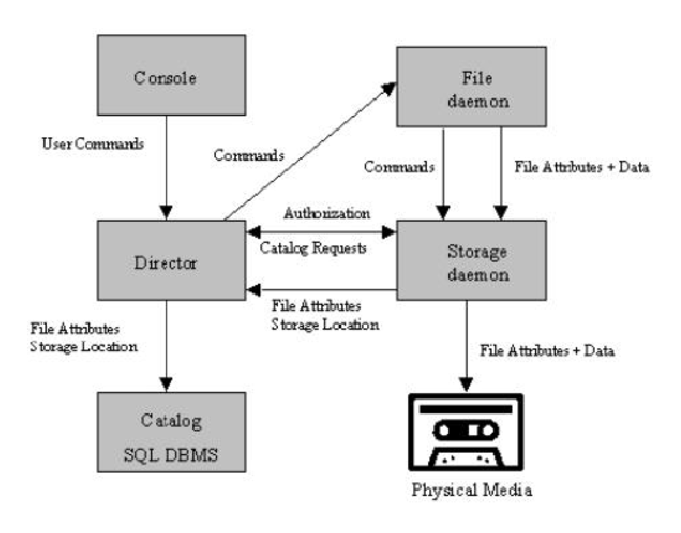
\includegraphics{./flow.eps} 
